\documentclass{beamer}
\usepackage[no-math]{fontspec}
\usepackage{xeCJK}
\setCJKmainfont{Source Han Sans TW}

\usetheme{CambridgeUS}
\title[OCT (Adhi \& Duker)]{Optical coherence tomography -- current and future applications}
\subtitle{Adhi \& Duker, \textit{Curr Opin Ophthalmol}, 2013}
\author[Chen-Pang He]{何震邦 (Chen-Pang He), M6 Clerk}
\date{Feb 7, 2018}

\institute[TMUH]
{
    Department of Ophthalmology\\
    Taipei Medical University Hospital
}

\begin{document}
\maketitle

\section{Introduction}
\begin{frame}{Key points}
    \begin{itemize}
        \item Choroid is implicated to be involved in the pathogenesis of
            retinal diseases, but until the advent of SD-OCT, its visualization
            was not feasible.
        \item Analysis of the choroid in healthy and diseased states such as
            AMD, CSCR, diabetic retinopathy and inherited retinal dystrophies
            has been successfully achieved using three commercially available
            SD-OCT systems.
        \item Longer wavelength OCT systems including the swept-source
            technology, Doppler OCT and en-face imaging, will help detect
            subtle microstructural changes in chorioretinal diseases.
    \end{itemize}
\end{frame}

\begin{frame}{Figure 1: Cirrus HD-OCT with image averaging}
    \begin{center}
        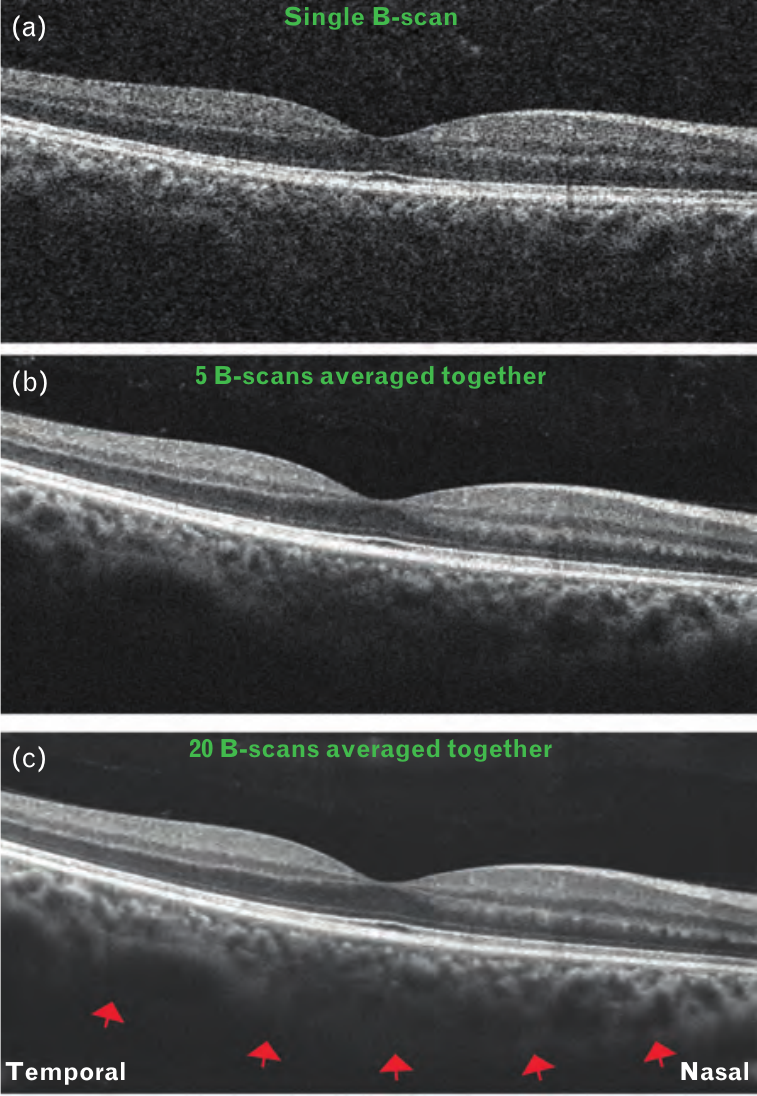
\includegraphics[height=0.8\textheight]{1.png}
    \end{center}
\end{frame}

\begin{frame}{Figure 2: enhanced depth imaging (EDI)}
    \begin{center}
        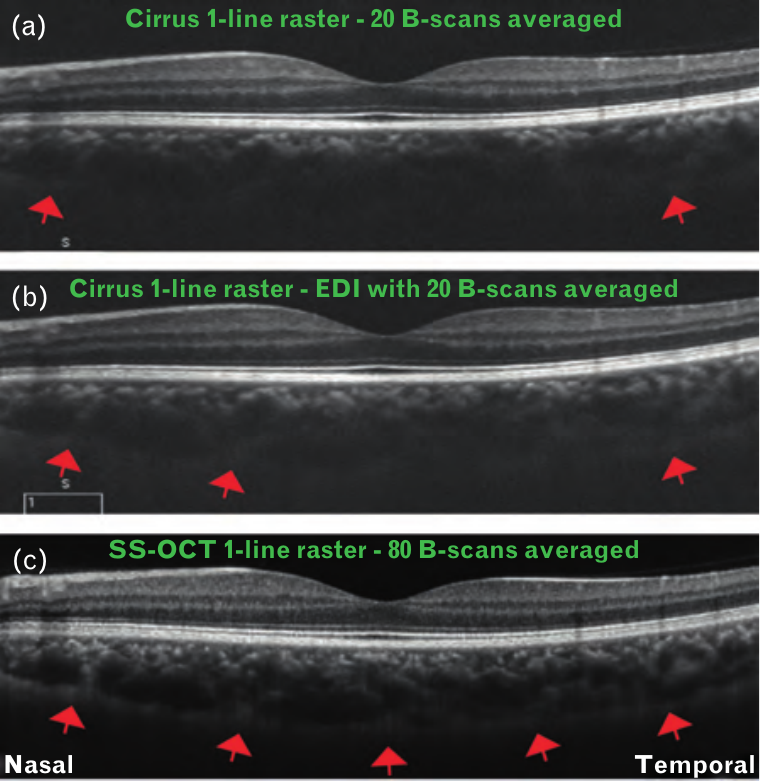
\includegraphics[height=0.8\textheight]{2.png}
    \end{center}
\end{frame}

\section{Present applications}
\begin{frame}{Figure 3: choroidal thickness of a healthy eye}
    \begin{center}
        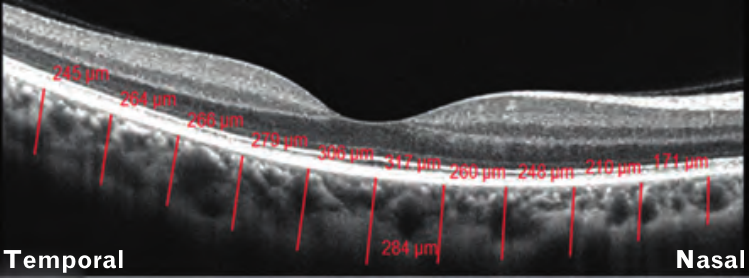
\includegraphics[width=\textwidth]{3.png}
    \end{center}
\end{frame}

\begin{frame}{Figure 4: differential diagnosis with choroidal thickness}
    \begin{center}
        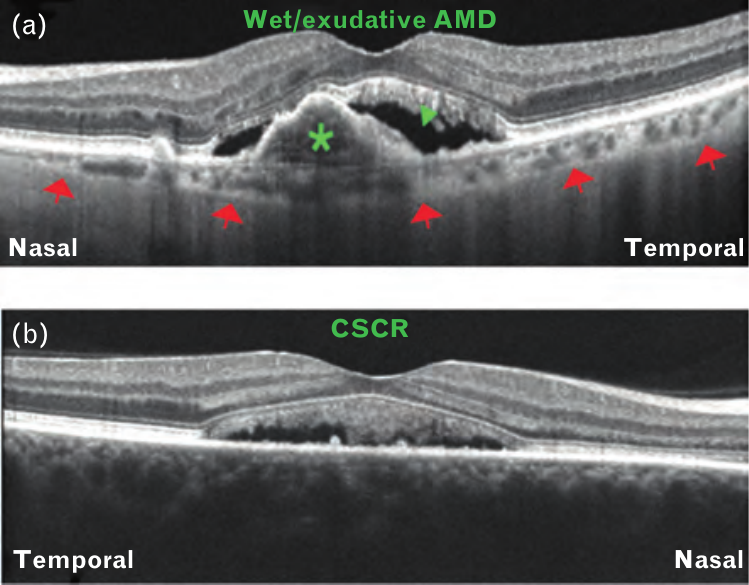
\includegraphics[height=0.8\textheight]{4.png}
    \end{center}
\end{frame}

\begin{frame}{Figure 5: choroidal thinning following anti-VEGF therapy}
    \begin{center}
        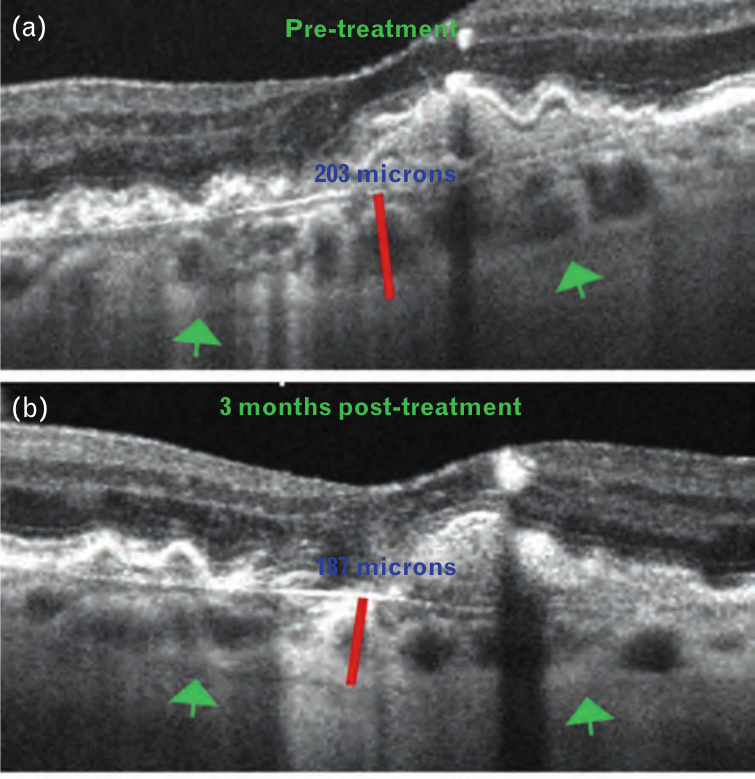
\includegraphics[width=0.46\textwidth]{5a.png}
        \quad
        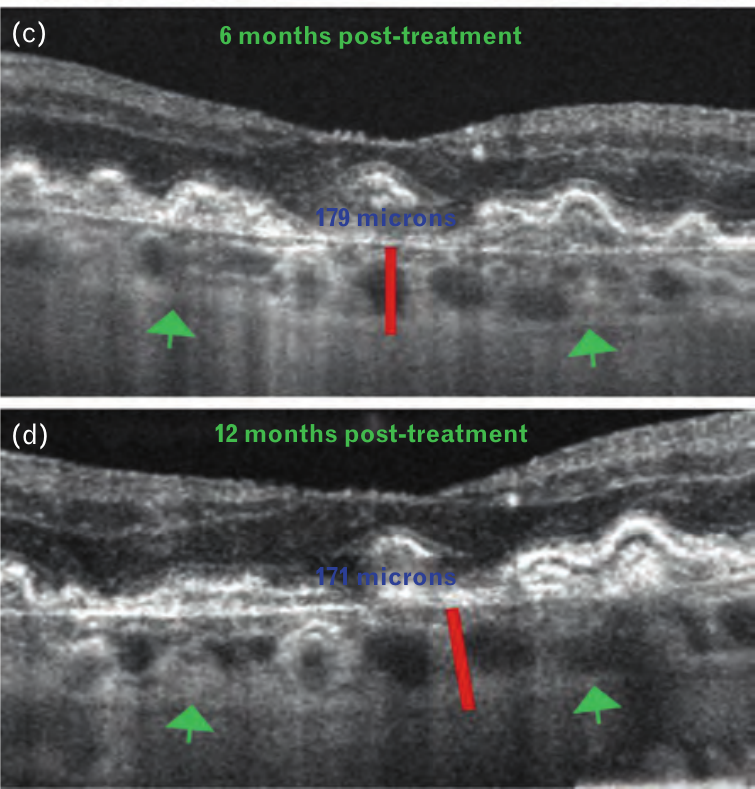
\includegraphics[width=0.46\textwidth]{5c.png}
    \end{center}
\end{frame}

\begin{frame}{Figure 6: diabetic retinopathy}
    \begin{center}
        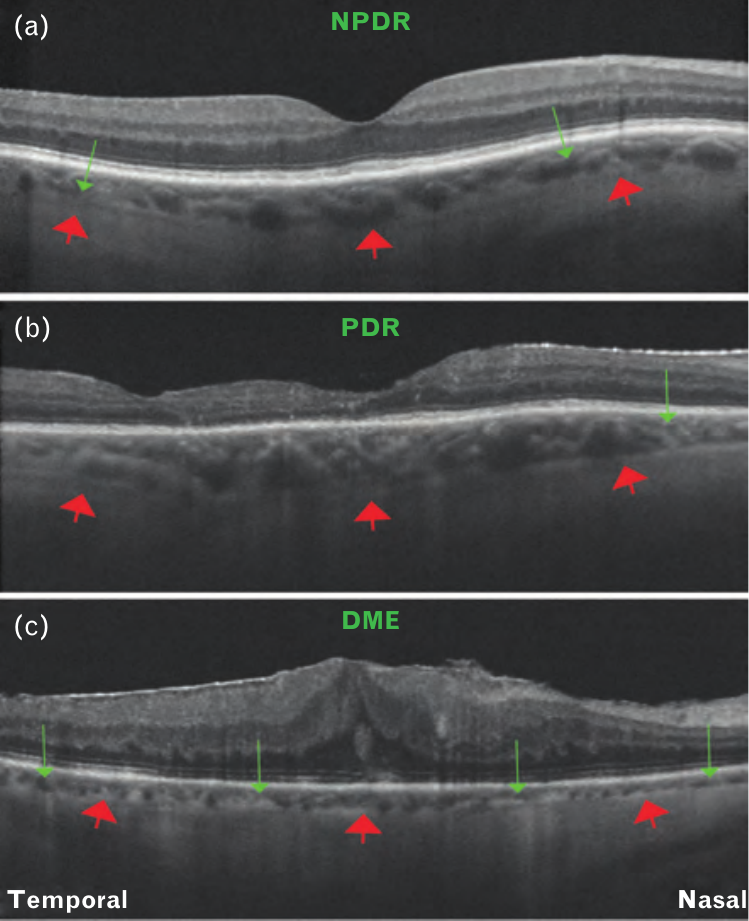
\includegraphics[height=0.8\textheight]{6.png}
    \end{center}
\end{frame}

\begin{frame}{Figure 7: inherited retinal dystrophies}
    \begin{center}
        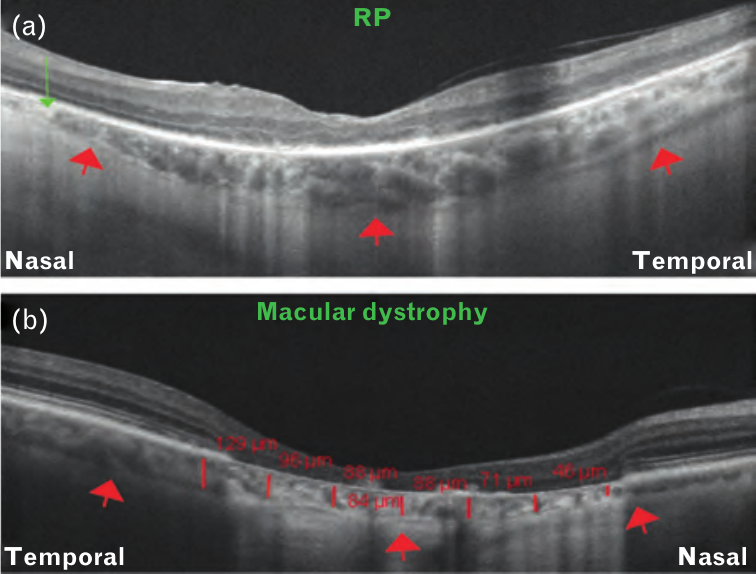
\includegraphics[height=0.8\textheight]{7.png}
    \end{center}
\end{frame}

\begin{frame}{Figure 8: choroidal osteoma}
    \begin{center}
        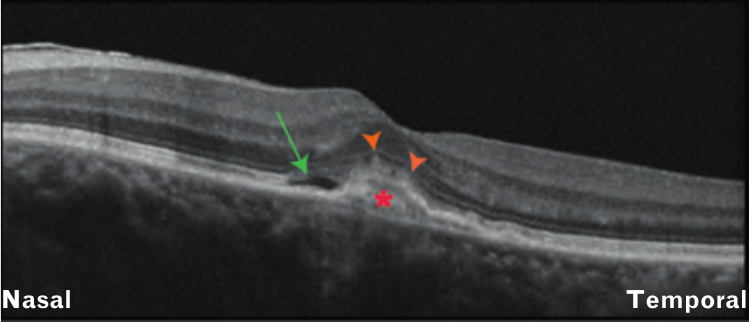
\includegraphics[width=\textwidth]{8.png}
    \end{center}
\end{frame}

\section{Future directions}
\begin{frame}{Future directions}
    \begin{itemize}
        \item Longer wavelength and swept source technology
        \item Doppler optical coherence tomography
        \item En-face imaging
    \end{itemize}
\end{frame}
\end{document}
